\documentclass[12pt]{article}
\usepackage{graphics}
\usepackage[top=1in,bottom=1in,left=1in,right=1in]{geometry}
\usepackage{alltt}
\usepackage{array}	
\usepackage{graphicx}
\usepackage{tabularx}
\usepackage{verbatim}
\usepackage{setspace}
\usepackage{listings}

\usepackage{amssymb,amsmath, amsthm}
\usepackage{zed-csp}
\usepackage[cc]{titlepic}

\title{COMP 335: Introduction to Theoretical Computer Science\\
\ \\
Assignment 6}
\author{Nathan Grenier}
\date{\today \\ Fall 2024}

\begin{document}
\begin{spacing}{1.5}
      \maketitle

      \newpage

      \begin{enumerate}

            \item[1.] [30 Points] Classify the following languages into one of the three categories:
                  \begin{enumerate}
                        \item regular
                        \item context-free but not regular
                        \item not context-free
                  \end{enumerate}
                  Prove your answer. Note that in order to show that a language is context-free but not regular, you need to prove both that it is context-free and also that it is not regular.

                  \begin{enumerate}
                        \item[(a)] $L_1 = \{a^ib^jc^k | k=i\times j \text{ and } 0 < i < 10 < j\}$

                              \textbf{Showing that $L_1$ is context-free:}
                              Since $i$ is bounded by a finite amount, we can construct individual grammars that accept the language for every specific $i$. Then we can combine all of these grammars into a single grammar that accepts the language $L_1$.

                              When $i=1$: $G_1=$
                              \begin{align*}
                                    S & \rightarrow aB            \\
                                    B & \rightarrow b^{11}Cc^{11} \\
                                    C & \rightarrow bCc|\lambda   \\
                              \end{align*}

                              When $i=2$: $G_2=$
                              \begin{align*}
                                    S & \rightarrow aaB           \\
                                    B & \rightarrow b^{11}Cc^{22} \\
                                    C & \rightarrow bCcc|\lambda  \\
                              \end{align*}

                              $\dots$

                              When $i=9$: $G_9=$
                              \begin{align*}
                                    S & \rightarrow a^9B          \\
                                    B & \rightarrow b^{11}Cc^{99} \\
                                    C & \rightarrow bCc^9|\lambda \\
                              \end{align*}

                              Finally, $G_1 \cup G_2 \cup \dots \cup G_9 = G_{f}:$
                              \begin{align*}
                                    S   & \rightarrow G_1 | G_2 | \dots | G_9 \\
                                    G_1 & \rightarrow \dots                   \\
                                    G_2 & \rightarrow \dots                   \\
                                    \dots                                     \\
                                    G_9 & \rightarrow \dots                   \\
                              \end{align*}

                              \textbf{Showing that $L_1$ is not regular:} We can use the pumping lemma for regular languages to prove that $L_1$ is not regular.

                              Let $m$ be the integer if the PL.

                              $$w = a^ib^{11+m}c^{i(11 + m)}$$
                              \begin{itemize}
                                    \item $w \in L_1$
                                    \item $|w|=i(11+m)+m+11+i. \therefore |w| \geq m$
                              \end{itemize}

                              By PL $\exists x,y,z : w = xyz, |xy| \leq m, |y| \geq 1$

                              $$|--i---|-|-m--|i(11+m)|$$
                              $$w_j=(aa\dots aa)b^{11}(bb\dots bb)(ccc\dots ccc)$$
                              $$|---xy-----|--z----|$$

                              Let $j=2$:
                              $w_2=xyyz=a^ib^{m-(11+i)}b^kb^{11+i}c^{i(11+m)}=a^ib^{m+k}c^{i(11+m)}$

                              \begin{itemize}
                                    \item $w_2 \in L_1 \text{ by PL}$
                                    \item $w_2 \not\in L_1 \text{ by the definition of }L_1.$ $n_a(w) \times n_b(w)=n_c(w) \text{ but } i(m+k) \not=i(11+m)$
                              \end{itemize}

                              \newpage
                        \item[(b)] $L_2 = \{xyz | x,y,z \in \{a,b \}^* \text{ and } n_a(x)=n_b(z) \}$

                              \textbf{Answer:} $L_2$ is a regular language.

                              \textbf{Proof:} There is a redundancy in the definition of language $L_2$. Since $x,y,z \in \{a,b\}^*$, all strings in the alphabet $\Sigma$ can be generated by only one of the 3 variables. Therefore, if we make $x,z = \lambda$, the language can still generate all possible strings in $\Sigma^*$ through $x$ and the condition of $n_a(x)=n_b(z)$ is true because $0=0$.
                              \\
                              \\
                              We can now construct a regular grammar $G$ that accepts the language $L_2=\{x | x \in \{a,b\}^* \text{ where } n_a(x)=n_b(z)\}$.

                              $G =$ \\
                              $S \rightarrow aS | bS | \lambda$

                              \newpage
                        \item[(c)] $L_3 = \{wuw^R | w,u \in \{a,b\}^* \text{ and } |w|=|u| \}$

                              \textbf{Answer:} $L_3$ is not a context-free language.

                              \textbf{Proof:}
                              \begin{figure}[h!]
                                    \centering
                                    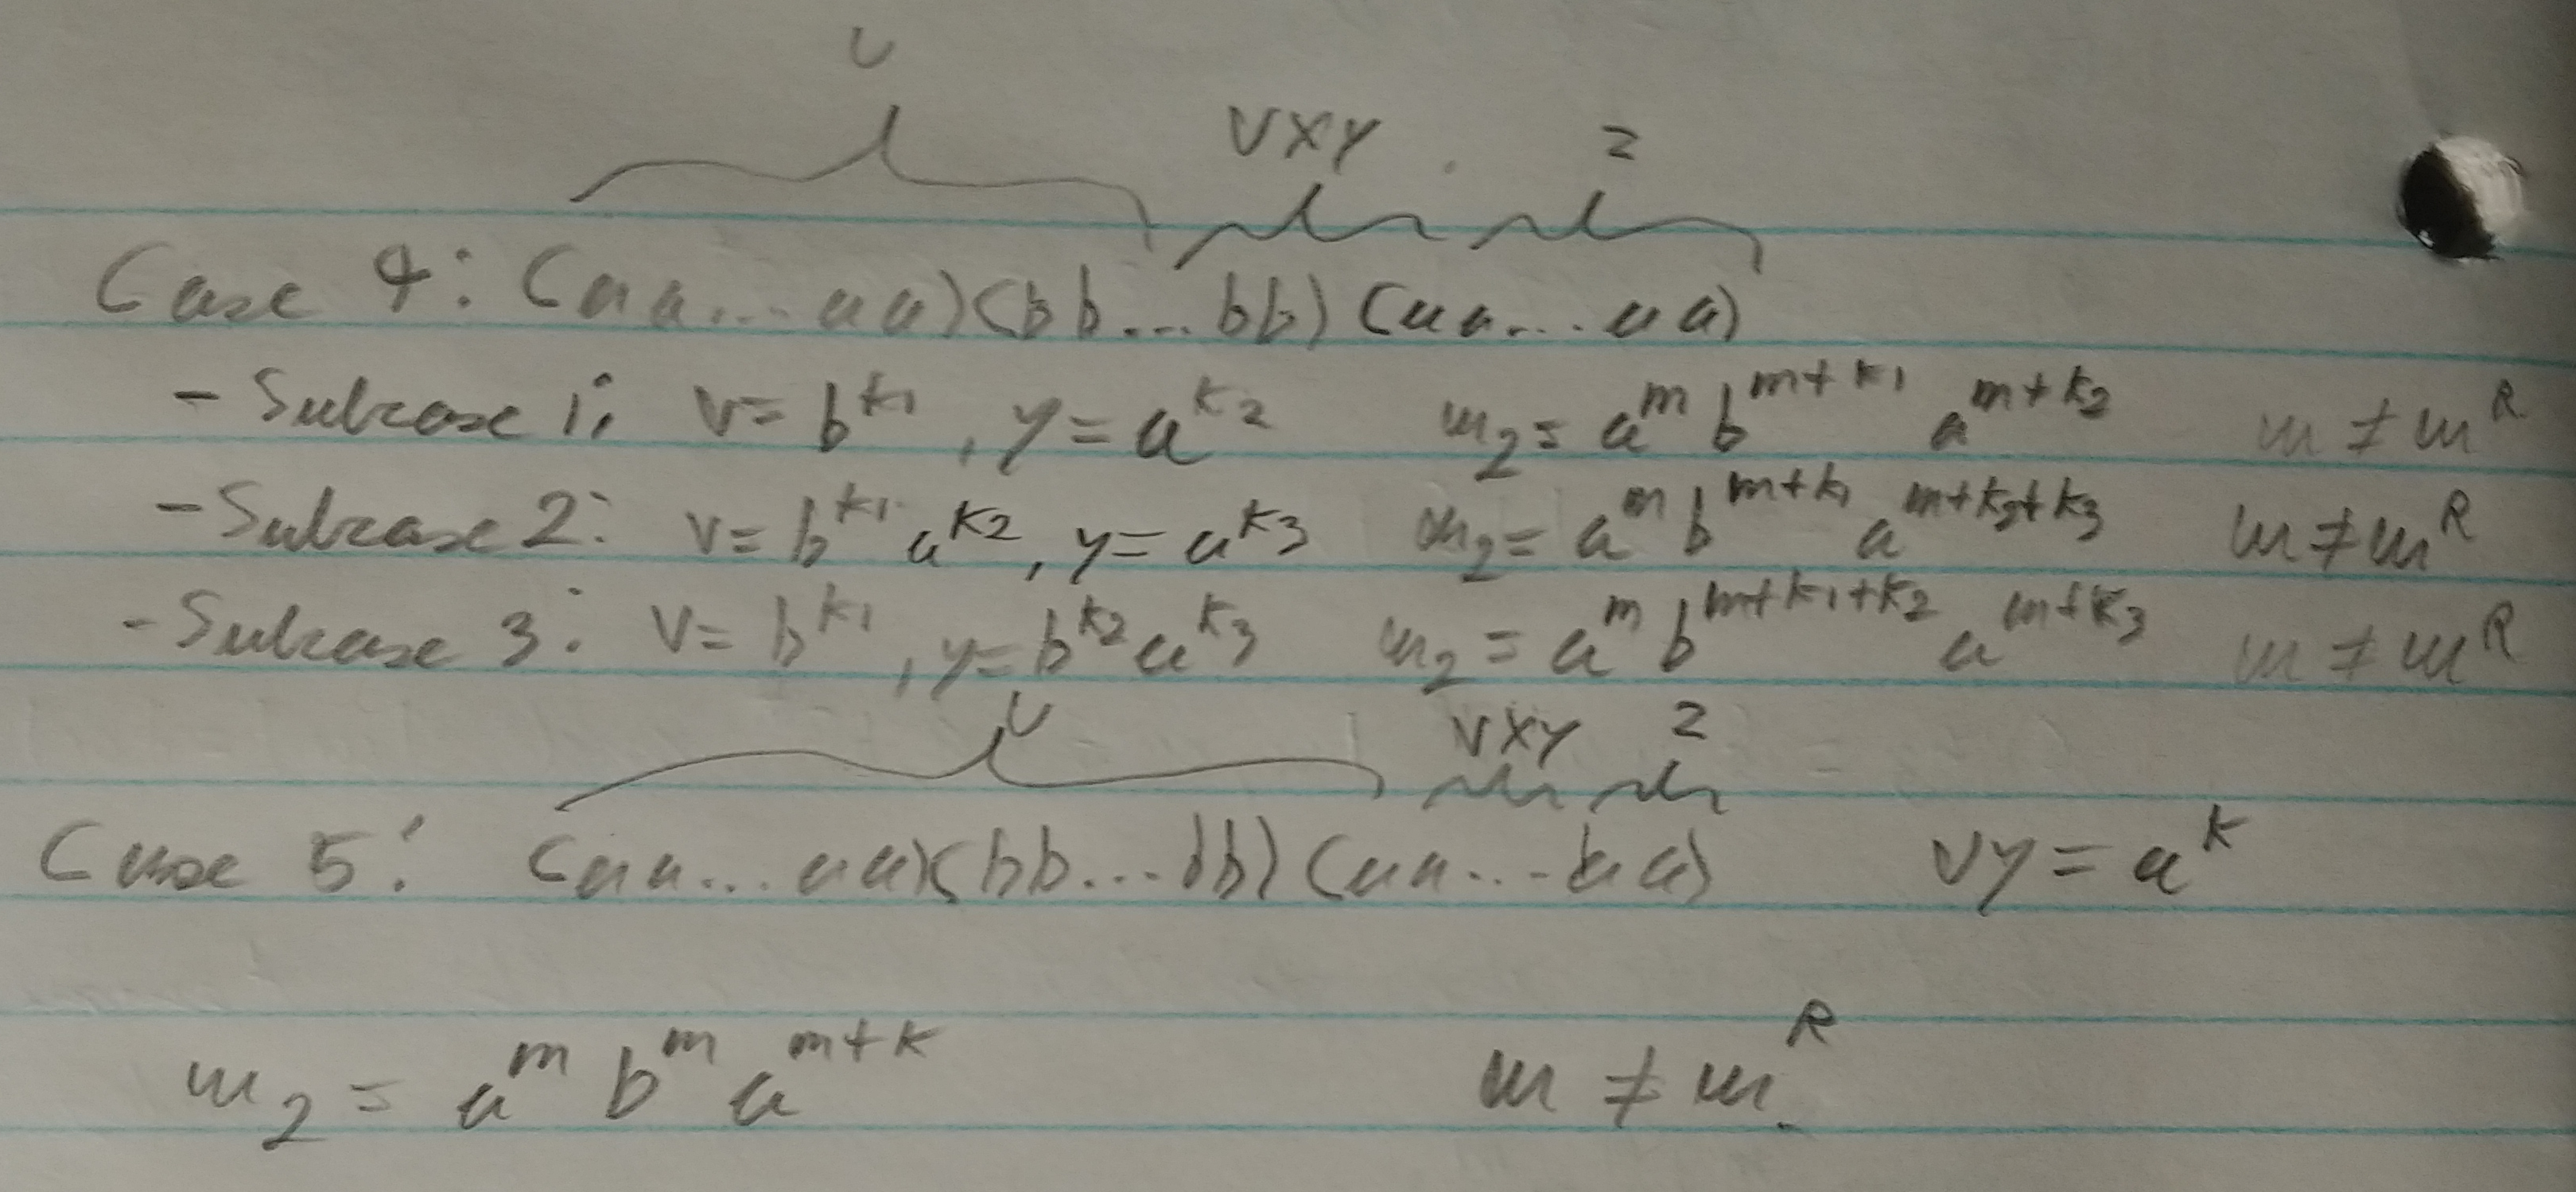
\includegraphics[width=0.7\textwidth]{img/q1/q1c_1.png}
                              \end{figure}
                              \begin{figure}[h!]
                                    \centering
                                    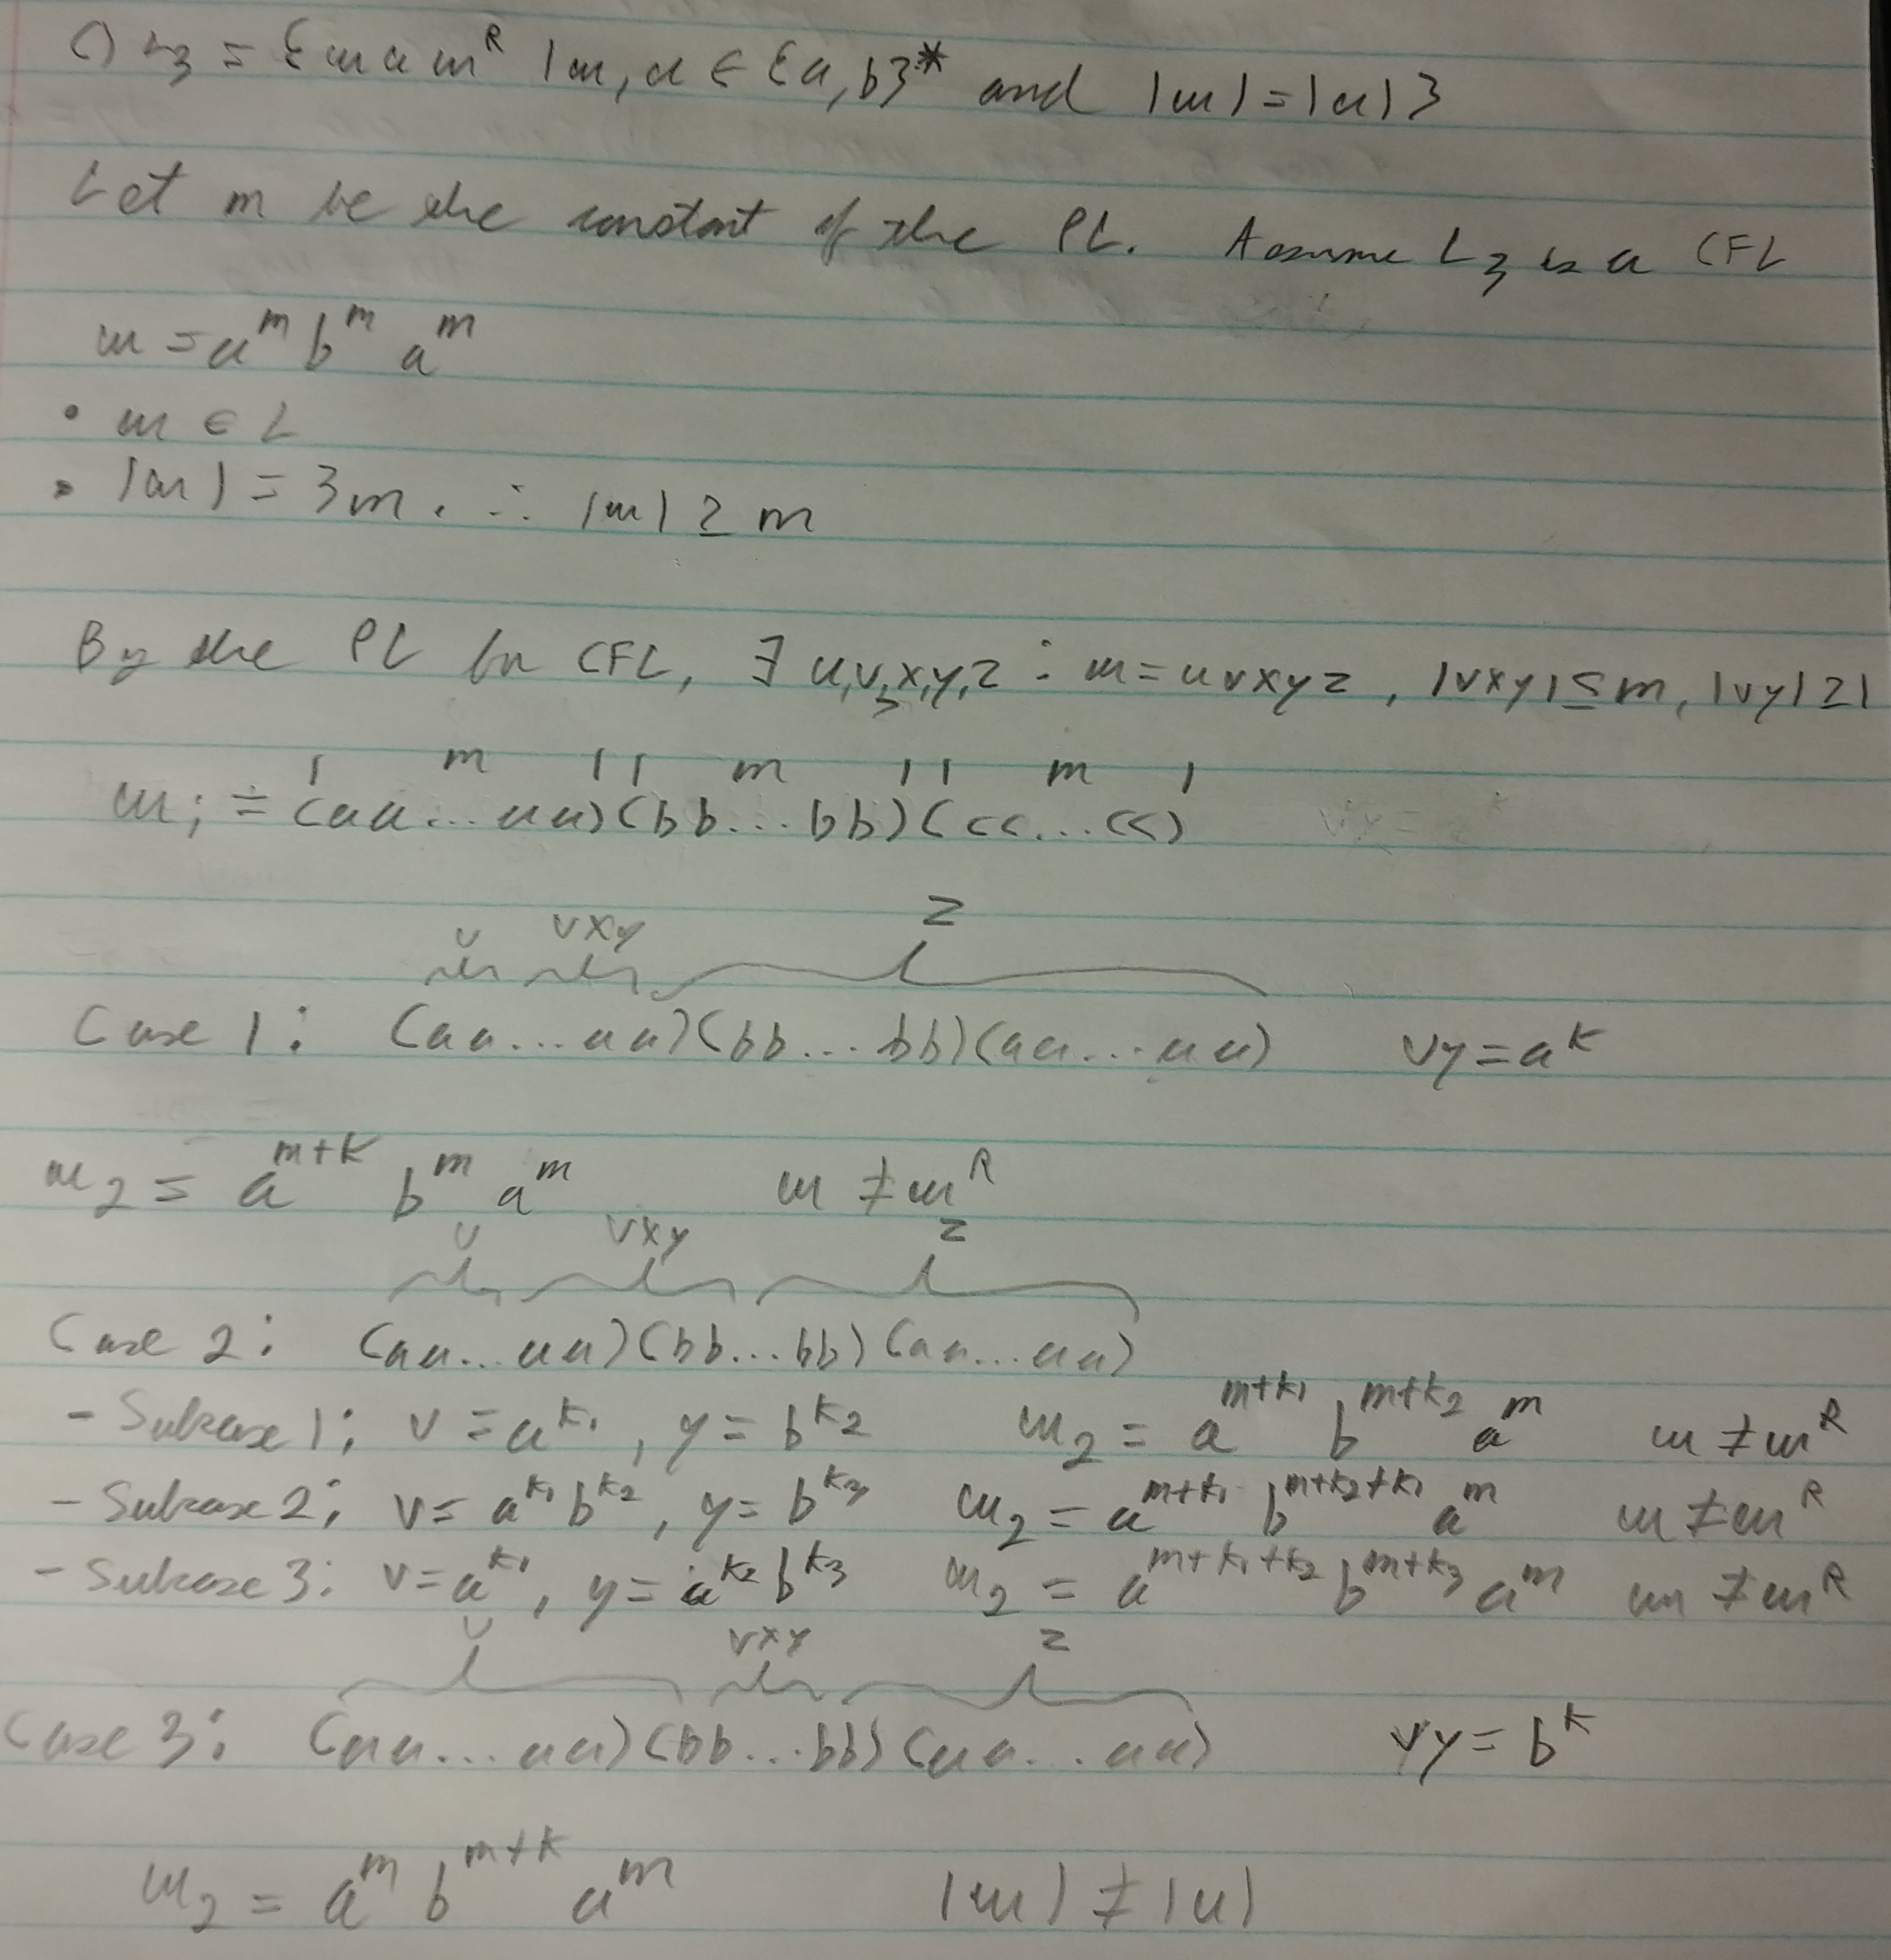
\includegraphics[width=0.7\textwidth]{img/q1/q1c_2.png}
                              \end{figure}
                  \end{enumerate}

                  \newpage
            \item[2.] [10 Points] Give a Turing machine for $L=\{a \} \cdot \{a,b \}^+$ that does not halt on rejection.

                  \begin{figure}[h!]
                        \centering
                        \includegraphics[width=0.7\textwidth]{img/q2/q2.png}
                  \end{figure}

                  \newpage
            \item[3.] [20 Points] Give a Turing machine for each of the following languages.

                  \begin{enumerate}
                        \item[(a)] $L_1 = \{a^nb^mc^k | m \geq n, k \geq 1 \}$

                              \begin{figure}[h!]
                                    \centering
                                    \includegraphics[width=0.7\textwidth]{img/q3/q3a.png}
                              \end{figure}

                        \item[(b)] $L_2 = \{xy | x \in \{a,b \}^+, y \in \{c\}^+ \text{ and } n_a(x)=n_c(y) \}$

                              \begin{figure}[h!]
                                    \centering
                                    \includegraphics[width=0.8\textwidth]{img/q3/q3b.png}
                              \end{figure}

                  \end{enumerate}

                  \newpage
            \item[4.] [20 Points] Draw transition diagrams for Turing machines that compute the following functions. In each case, give a brief description in English of your solution strategy.

                  \begin{enumerate}
                        \item[(a)] $f(1^n) = 1^{2n}$

                              \textbf{Algorithm Description:}
                              The algorithm is as follows:
                              \begin{enumerate}
                                    \item Iterate over the initial number, replacing every $1$ with an $x$.
                                    \item Once we reach the end of the string, use the zig zag pattern to replace every $x$ with a $1$ and simultaneously add a $1$ at the end of the string.
                                    \item When there are no more $x$s to replace we've successfully duplicated the entire input. Therefore we move the head to the start of the string and halt.
                              \end{enumerate}

                              Note that this algorithm can also handle the case where $n=0$. Since there are no $1$s to copy, the algorithm will terminate early in state $q_2$.

                              \begin{figure}[h!]
                                    \centering
                                    \includegraphics[width=0.6\textwidth]{img/q4/q4a.png}
                              \end{figure}

                              \newpage
                        \item[(b)] $f(1^n) = 1^{n^2}$

                              \textbf{Algorithm Description:}
                              A number to the power of 2 is the number multiplied by itself. Multiplication is a chain of additions. Example: $3^3 = 3\times 3 = 3 + 3 + 3$.

                              The algorithm is as follows:
                              \begin{enumerate}
                                    \item Copy the initial number to the right of the input string delimited by a $0$. This copy will be used for future additions / copies.
                                    \item Iterate over the initial number, replacing every $x$ with a $\$$.Each $\$$ represents the number of times the initial number needs to be copied (added).
                                    \item Now, iterate over the $\$$s and copy the copy of the initial number for as many times as there are $\$$ characters (each copy is delimited by a $0$). We replace $\$$ that have already been iterated on with $Z$. Note that we mark off an extra $\$$ at the start since we've already copied the initial number once.
                                    \item Once there are no more $\$$s, we erase the iterators and it's delimiter.
                                    \item Finally, we clean up the computed string. First we replace all $x$s with $1$s. Then we remove all delimiters by replacing them with $1$ and removing a $1$ at the end of the string.
                                    \item We then move the head to the start of the string and halt.
                              \end{enumerate}

                              Note that there are certain edge cases that must be handled:
                              \begin{itemize}
                                    \item $1^2=1$: Therefore we must terminate early in state $q_{10}$.
                                    \item $0^2=0$: Therefore we must terminate early in state $q_3$.
                              \end{itemize}

                              \begin{figure}[h!]
                                    \centering
                                    \includegraphics[width=1\textwidth]{img/q4/q4b.png}
                              \end{figure}

                  \end{enumerate}

      \end{enumerate}

\end{spacing}

\end{document}